\documentclass{article}
\usepackage[utf8]{inputenc}
\usepackage{amssymb}
\usepackage{listings}
\usepackage{color}
\usepackage{titleps}

\newpagestyle{mystyle}{
	\sethead[\thepage][\Author][]{}{\Author}{\thepage}
}
\pagestyle{mystyle}

\author{First Author \and Second Author}
\title{The title}

\makeatletter
\newcommand\Author{Jan Odermatt}
\let\Title\@title
\makeatother

\usepackage{geometry}
\geometry{left=10mm, right=10mm, top=15mm, bottom=15mm}
\usepackage{graphicx}
\usepackage{float}
\usepackage{amsmath}
\usepackage{blindtext}
\graphicspath{ {./bilder/} }
\renewcommand{\baselinestretch}{2}
\author{Jan Odermatt}
\title{Zusammenfassung Machinelearning}
\begin{document}
\tableofcontents
\section{Machine Learning Grundlagen}
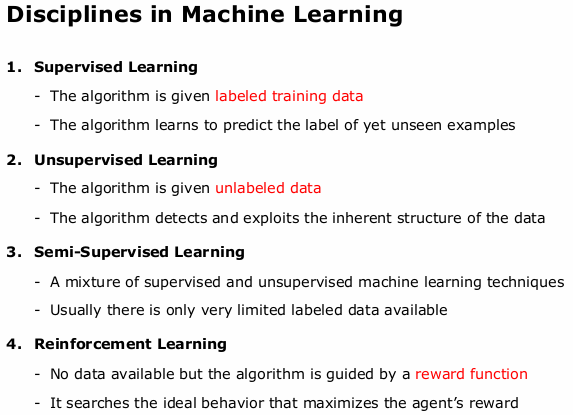
\includegraphics[width=0.4\textwidth]{disciplines_in_machine_learning.png}
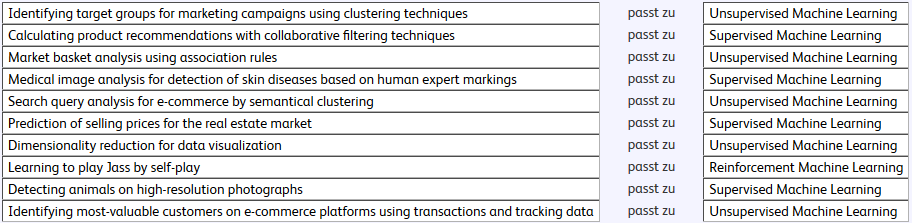
\includegraphics[width=0.6\textwidth]{disciplines_matched.png}
\section{Data Quality Assessment}
	\begin{enumerate}
		\item Data Cleaning\footnote{Auch wenn die Datenqualität selbständig verbessert werden kann sollten: alle Änderungen dokumentiert werden, data-repository mit versionierung verwendet werden, den Herausgeber der Daten auf fehler in den Daten hinweisen}
		\begin{enumerate}
			\item Dublizierte Daten erkennen und entfernen
			\item Daten mit nullen können ersetzt werden.
			\item Daten Machine Learning freundlicher gestalten (z.B. für Farben eigene Zeilen erstellen, damit die Euklid-Distanz gerechnet werden kann.
		\end{enumerate}
		\item Analyse mit Hilfe von
		\begin{enumerate}
		\item 5 Nummer Zusammenfassung (median Q2, Quartile Q1 und Q3 sowie min und max)
		\item Boxplots um das Datenset auf Ausreisser zu prüfen.
		\item Varianz und Standardabweichung berechnen
		\end{enumerate}
	\end{enumerate}
\section{Machine Learning Fundamentals}
	\begin{tabular}{c c c}
	  Euklid Distanz & Kosinus Ähnlichkeit & Formel Kosinus Similarity\\
    	  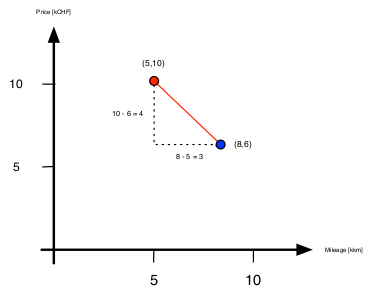
\includegraphics[width=0.25\linewidth]{euclide_distance.png} & 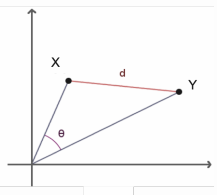
\includegraphics[width=0.25\linewidth]{cosine_similarity.png} & 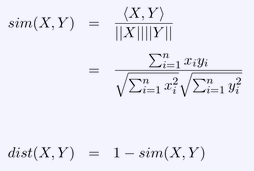
\includegraphics[width=0.25\linewidth]{cosine_similarity_formula.png} \\
	\end{tabular}
\section{Supervised Learning Basics}
\begin{tabular}{l l}
	\parbox[c]{0.3\textwidth}{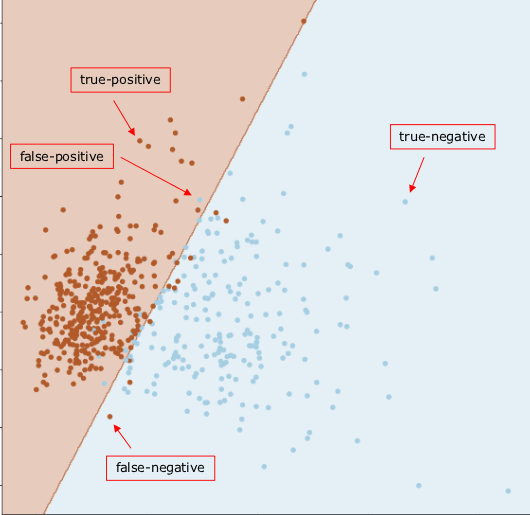
\includegraphics[width=\linewidth]{true_positive}} &
	\begin{tabular}{l}
		$Accuracy = \frac{TP + TN}{Total}$ \\ $Errorrate = \frac{FP + FN}{Total}$ \\
		$Sensitivity = \frac{TP}{Actual Yes}$ = $\frac{TP}{TP + FN}$ \\ $Specificity = \frac{TN}{ActualNo} = \frac{TN}{TN + FP}$ \\ 
		$Precision = \frac{TP}{Predicted Yes} = \frac{TP}{TP + FP}$
	\end{tabular}
	
\end{tabular}
\section{Linear Regression}
	Das Modell hat generell die folgende Form: $y = h_\theta(x) = \theta_0 + \theta_1 x$.
	
	Mit $\bar{x}$ und $\bar{y}$ als Mittelwerte der Datenreihe, können somit die Werte $\theta_1$ und $\theta_0$ berechnet werden. \footnote{Bei $var^{(i)}$ ist $i$ ein Index für den Datenpunkt und kein Exponent.}
	\[ \theta_1 = \frac{\sum_{i=1}^{n}(y^{(i)}-\bar{y})(x^{(i)}-\bar{x})}{\sum_{i=1}^{n}(x^{(i)}-\bar{x})} = \frac{S_{xy}}{S_{xx}} \qquad
	\theta_0 = \bar{y}-\theta_1 \bar{x} \]

\section{Gradient Descent}
	Mit der Kostenfunktion $$J(\theta) = \frac{1}{2 n} \sum_{i=1}^{n}(h(\theta,x^{(i)})-y^{(i)})^2$$ wo $h(\theta,x^{(i)})$ die Vorhersage von $y$ ist und als $$h(\theta_k,x^{(i)})= (x^{(i)})^T\theta=\theta_0+\theta_1x_1^{(i)}+\theta_2x_2^{(i)}+...+\theta_mx_m^{(i)}$$
	ausgeschrieben wird, kann $\theta$ optimiert werden.	
	Diese wird mit $\theta = (X^T X)^{-1} X^T y$ umgesetzt. 
	In python wird das mit X als $n \times m$ Matrix, bei der die erste Spalte mit Einsen aufgefüllt wurde und mit y als Zielwert
	$\theta = 
	\begin{bmatrix}
	\theta_0 \\[0.1pt] \theta_1 \\[0.1pt] ... \\[0.1pt] \theta_m
	\end{bmatrix}$ definiert wird.
	
	\begin{lstlisting}
	theta = np.linalg.inv(X.T.dot(X)).dot(X.T).dot(y)
	\end{lstlisting}
	
	Korrelation liegt immer zwischen $-1 <= r <= 1$.
	$r = 0$ bedeutet keine Korrelation und $|r| = 1$ vollständige Korrelation.
\section{Logistische Regression (eigentlich Klassifikation)}
	Logistische Regression zielt darauf ab eine binäre Zuordnung vorzunehmen (z.B. Brustkrebs oder nicht; Spam-Mail oder nicht etc.).
	Dabei können die unabhängigen Variablen numerisch (12mm) oder kategorisch (mag Skifahren) sein.
	
	Die Logistische Funktion nennt sich auch "Siegmoid Funktion" und lautet wie folgt:
	$$\sigma(z) = \frac{1}{1+e^{-z}} = \frac{e^z}{e^z+1}, z \in \mathbb{R}$$
	Die Logistische Funktion ist auch die neue Hypothese: $$h_\theta(x)=\frac{1}{1+e^{\theta^Tx}}$$
	Die Ableitungen der Logistischen Funktion sehen folgendermassen aus.
	$$\sigma^{\prime}(x) = \sigma(z) (1-\sigma(z))$$
	$$\sigma^{\prime\prime}(z)= \sigma(z)(1-\sigma(z))(1-2\sigma(z))$$
	
	Wenn $z > 0$ wird die Aussage als wahr (Wahrscheinlichkeit über 0.5) und sonst als falsch interpretiert.
	
	$z$ ist mit $z=\theta^T x = \theta_0 + \theta_1 x_1 + \theta_2 x_2$ gegeben.
	
	Mit der Logistischen Regression muss auch eine neue Kostenfunktion gewählt werden, welche folgendermassen aussieht:
	$$Cost(h_\theta(x), y) = \begin{cases}
	-log(h_\theta(x)) & wenn\;y = 1 \\
	-log(1-h_\theta(x)) & wenn\;y = 0
	\end{cases}$$
	Damit ergibt sich die Formel für Gradient Descent wie folgt:
	$$\theta_{k+1}=\theta_k-\alpha\frac{1}{n}X^T(\sigma(X\theta_k)-y)$$
	
	Codebeispiel zum trainieren von $\theta$
	\begin{lstlisting}
	def sigmoid(z):
		return 1/(1+np.exp(-z))
	
	def cost_function(X, y, theta):
		y_hat = sigmoid(np.dot(X,theta))
		J_i =-y*np.log(y_hat)-(1-y)*np.log(1-y_hat)
		J = J_i.sum()/len(y)
		return J
	
	def update_theta(X,y, theta, alpha):
		theta -= alpha * np.dot(X.T,sigmoid(np.dot(X, theta))-y)/len(y)
		return theta
	
	def train(X, y, theta, alpha, kmax):
		cost_history=[]
		for i in range(kmax):
			theta=update_theta(X,y,theta,alpha)
			cost = cost_function(X,y,theta)
			cost_history.append(cost)
		return theta, cost_history
	\end{lstlisting}
	Danach wird zuerst ein $\theta$ definiert, wo die vorgegebenen startwerte angegeben werden. Daraus trainiert der Algorythmus danach mit $\alpha$ als Schrittgrösse und \textbf{kmax} als Anzahl Zyklen die optimalen Werte für $\theta$
\end{document}
